% Generated by gen_fig6_wikimedia_fixture_drift.py
\begin{figure*}[t]
  \centering
  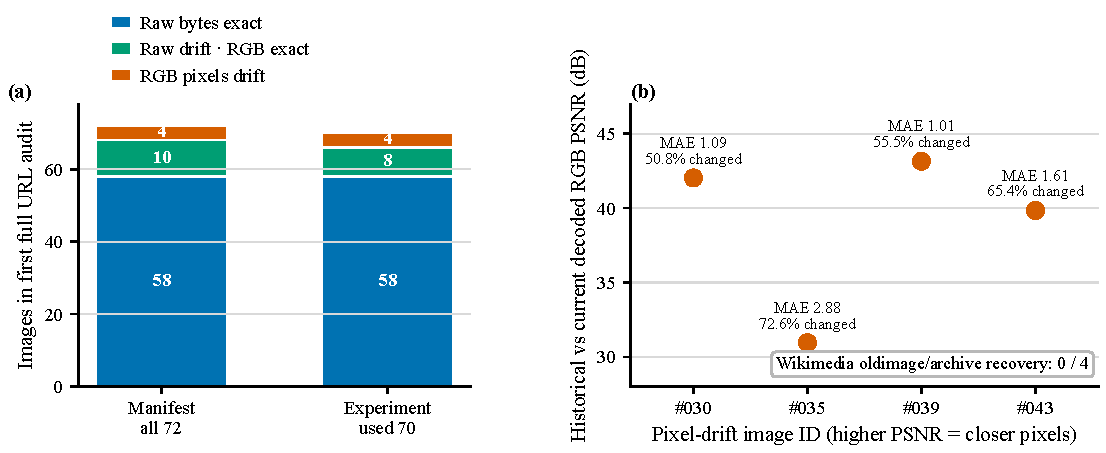
\includegraphics[width=\textwidth]{figures/fig6_wikimedia_fixture_drift.pdf}
  \caption{Mutable-upstream audit of the historical 72-image Wikimedia fixture. (a) Only 58 responses remained byte-identical; ten changed only JPEG metadata while preserving decoded RGB, and four changed decoded pixels. (b) The four pixel-drift cases differ measurably despite unchanged dimensions. No historical raw or pixel-drift input was recovered through Wikimedia oldimage/archive. The existing experiment keeps its historical raw-SHA provenance and the downloader fails closed; exact fresh-clone replay requires a separately licensed content-addressed archive or a new experiment ID. The public artifact freezes historical pins and the audit summary, not transient current-response binaries or the complete per-file archive transcript; current-side differences are contemporaneous audit-record observations rather than independently offline-replayable measurements.}
  \label{fig:wikimedia-fixture-drift}
\end{figure*}
\begin{table*}[t]
\centering
\caption{Reconstruction audit for the mutable Wikimedia thumbnail URLs used by the historical preference-study fixture. Percentages describe one sequential full pass on 2026-08-29; they are not availability guarantees.}
\label{tab:wikimedia-fixture-drift}
\small
\begin{tabular}{lrrrr}
\toprule
Scope & Raw exact & Raw drift / RGB exact & RGB drift & Archive recovery \\
\midrule
All manifest images ($n=72$) & 58 (80.56\%) & 10 (13.89\%) & 4 (5.56\%) & raw 0 / 14; pixels 0 / 4 \\
Experiment-used images ($n=70$) & 58 (82.86\%) & 8 (11.43\%) & 4 (5.71\%) & raw 0 / 12; pixels 0 / 4 \\
\bottomrule
\end{tabular}
\end{table*}

